\documentclass{article}
\usepackage{graphicx}
\usepackage{listings}
\usepackage{flexisym}

\graphicspath{ {images/} }

\newcommand{\overbar}[1]{\mkern 1.5mu\overline{\mkern-1.5mu#1\mkern-1.5mu}\mkern 1.5mu}

\begin{document}

  \title{CS 321: Assignment 6}
  \author{Jared Wasinger}

  \maketitle

	\begin{enumerate}
		\item Answer \begin{enumerate}
				\item \textbf{Base Case:} 
					$w = \epsilon$\\
					$\delta^*(s,w) = \delta^*(s, \epsilon) = q$\\
					$ A_s \rightarrow^* wA_q, A_S \rightarrow cA_q, A_s \rightarrow \epsilon A_q$\\

				\textbf{Inductive Step:}\\
					Let $w = xb$\\
					$\delta(\delta^*(s, x), b) = q$\\
					Let p = $\delta^*(s, x)$\\
					$\delta(p, b) = q$\\
					$A_s \rightarrow xA_p, A_p \rightarrow bA_q$\\
					$A_s \rightarrow^* xbA_q, A_s \rightarrow^* wA_q$\\

				L(DFA) = L(CFL)\\
					$L(DFA) = \{ w | \delta^*(s,w) \in F\}$\\
					$L(CFL) = \{ w | A_s \rightarrow^* w\}$\\
					An accepted string w must end in a terminal which means $w \in F$ as per the production rules of the given CFG.
				\item 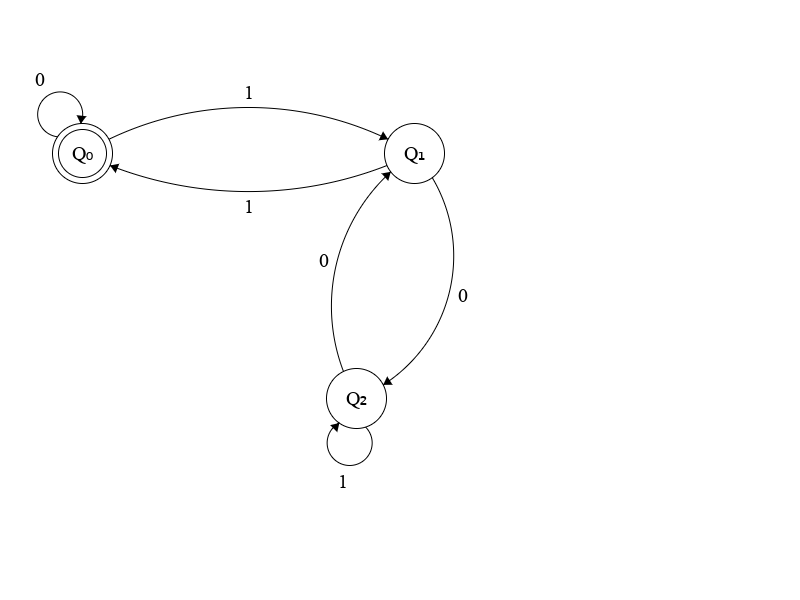
\includegraphics[width=\textwidth]{p1_b.png}\\
					\begin{itemize}\textbf{Derivation of CFG:}\\
						\item Starting nonterminal $A_s$
						\item $A_s \rightarrow 0A_s | 1A_1 | \epsilon$
						\item $A_1 \rightarrow 1A_s | 0A_2$
						\item $A_2 \rightarrow 1A_2 | 0A_1$
					\end{itemize}
			\end{enumerate}
		
		\item 
			$S \rightarrow aSddd | T$\\
			$T \rightarrow bTdd | R$\\
			$R \rightarrow cR | \epsilon$\\
			\begin{enumerate}
			\item \textbf{Eliminate the start symbol from right-hand sides}\\
				$S_0 \rightarrow S$\\
				$S \rightarrow aSddd | T$\\
				$T \rightarrow bTdd | R$\\
				$R \rightarrow cR | \epsilon$\\
			\item \textbf{TERM: Eliminate rules with nonsolitary terminals}\\
				
				$S_0 \rightarrow S$\\
				$S \rightarrow S_1SS_2S_3S_4 | T$\\
				$T \rightarrow T_1TT_2T_3 | R$\\
				$R \rightarrow R_1R | \epsilon$\\\\
				$S_1 \rightarrow a$\\
				$S_2 \rightarrow d$\\$S_3 \rightarrow d$\\$S_4 \rightarrow d$\\\\
				$T_1 \rightarrow b$\\ $T_2 \rightarrow d$\\$T_3 \rightarrow d$\\\\
				$R_1 \rightarrow c$\\
				
			\item \textbf{BIN: Eliminate right-hand sides with more than 2 nonterminal }\\
				$S_5 \rightarrow S_1S$\\
				$S_6 \rightarrow S_2S_3$\\
				$S_7 \rightarrow S_5S_6$\\
				$S \rightarrow S_7S_4 | T$\\

				$S_1 \rightarrow a$\\
				$S_2 \rightarrow d$\\$S_3 \rightarrow d$\\$S_4 \rightarrow d$\\\\

				$T_4 \rightarrow T_1T$\\
				$T_5 \rightarrow T_2T_3$\\
				$T \rightarrow T_4T_5 | R$\\\\

				$T_1 \rightarrow b$\\ $T_2 \rightarrow d$\\$T_3 \rightarrow d$\\\\

				$R \rightarrow R_1R | \epsilon$\\\\
				$R_1 \rightarrow c$\\

			\item \textbf{DEL: Eliminate $\epsilon$-rules}\\
				$S_5 \rightarrow S_1S$\\
				$S_6 \rightarrow S_2S_3$\\
				$S_7 \rightarrow S_5S_6$\\
				$S \rightarrow S_7S_4 | T$\\

				$S_1 \rightarrow a$\\
				$S_2 \rightarrow d$\\$S_3 \rightarrow d$\\$S_4 \rightarrow d$\\\\

				$T_4 \rightarrow T_1T$\\
				$T_5 \rightarrow T_2T_3$\\
				$T \rightarrow T_4T_5 | R$\\\\

				$T_1 \rightarrow b$\\ $T_2 \rightarrow d$\\$T_3 \rightarrow d$\\\\

				$R \rightarrow R_1R | R_1$\\\\
				$R_1 \rightarrow c$\\
			\item \textbf{UNIT: Eliminate unit rules}\\
				No unit rules
			\item \textbf{Final Answer}\\
				$S_5 \rightarrow S_1S$\\
				$S_6 \rightarrow S_2S_3$\\
				$S_7 \rightarrow S_5S_6$\\
				$S \rightarrow S_7S_4 | T$\\

				$S_1 \rightarrow a$\\
				$S_2 \rightarrow d$\\$S_3 \rightarrow d$\\$S_4 \rightarrow d$\\\\

				$T_4 \rightarrow T_1T$\\
				$T_5 \rightarrow T_2T_3$\\
				$T \rightarrow T_4T_5 | R$\\\\

				$T_1 \rightarrow b$\\ $T_2 \rightarrow d$\\$T_3 \rightarrow d$\\\\

				$R \rightarrow R_1R | R_1$\\\\
				$R_1 \rightarrow c$\\
			\end{enumerate}
		\item Answer \begin{enumerate}
			\item This language has the following cases:
				\begin{itemize}
					\item$k=m, k \neq n$
					\item$m=n, n \neq k$
					\item$k=n, n \neq m$
					\item$k \neq m \neq n$
				\end{itemize}
			\item $S_0 \rightarrow SS_2$\\
				$S \rightarrow aSa | bSb | cS_2$\\
				$S_2 \rightarrow aS_2 | bS_2 | \epsilon$\\
		\end{enumerate}
	\end{enumerate}
\end{document}
